%%%%%%%%%%%%%%%%%%%%%%%%%%%%%%%%%%%%%%%%%%%%%%%%%%%%%%%%%%%%%%%%%%%%%%%%%%%%%%%%%%%%%%%%%%
% Ceci est le fichier principal du template template à utiliser pour les rapports du     %
% projet 2 (TAD) d'INFO0947.                                                             %
%                                                                                        %
% Vous devez décommenter et compléter les commandes introduites plus bas (intitule, ...) %
% avant de pouvoir compiler le fichier LaTeX.  Pensez à configurer votre Makefile en     %
% conséquence.                                                                           %
%                                                                                        %
% Le contenu et la structure du rapport sont imposés.  Vous devez compléter les          %
% différents fichiers .tex inclus dans ce fichier avec votre production.                 %
%%%%%%%%%%%%%%%%%%%%%%%%%%%%%%%%%%%%%%%%%%%%%%%%%%%%%%%%%%%%%%%%%%%%%%%%%%%%%%%%%%%%%%%%%%

% !TEX root = ./main.tex
% !TEX engine = latexmk -pdf
% !TEX buildOnSave = true
\documentclass[a4paper, 11pt, oneside]{article}

\usepackage[utf8]{inputenc}
\usepackage[T1]{fontenc}
\usepackage[french]{babel}
\usepackage{array}
\usepackage{shortvrb}
\usepackage{listings}
\usepackage[fleqn]{amsmath}
\usepackage{amsfonts}
\usepackage{fullpage}
\usepackage{enumerate}
\usepackage{graphicx}             % import, scale, and rotate graphics
\usepackage{subfigure}            % group figures
\usepackage{alltt}
\usepackage{url}
\usepackage{indentfirst}
\usepackage{eurosym}
\usepackage{listings}
\usepackage{color}
\usepackage[table,xcdraw,dvipsnames]{xcolor}
\usepackage{multirow}

\definecolor{mygray}{rgb}{0.5,0.5,0.5}
\newcommand{\coms}[1]{\textcolor{MidnightBlue}{#1}}

\lstset{
    language=C, % Utilisation du langage C
    commentstyle={\color{MidnightBlue}}, % Couleur des commentaires
    frame=single, % Entoure le code d'un joli cadre
    rulecolor=\color{black}, % Couleur de la ligne qui forme le cadre
    stringstyle=\color{RawSienna}, % Couleur des chaines de caractères
    numbers=left, % Ajoute une numérotation des lignes à gauche
    numbersep=5pt, % Distance entre les numérots de lignes et le code
    numberstyle=\tiny\color{mygray}, % Couleur des numéros de lignes
    basicstyle=\tt\footnotesize,
    tabsize=3, % Largeur des tabulations par défaut
    keywordstyle=\tt\bf\footnotesize\color{Sepia}, % Style des mots-clés
    extendedchars=true,
    captionpos=b, % sets the caption-position to bottom
    texcl=true, % Commentaires sur une ligne interprétés en Latex
    showstringspaces=false, % Ne montre pas les espace dans les chaines de caractères
    escapeinside={(>}{<)}, % Permet de mettre du latex entre des <( et )>.
    inputencoding=utf8,
    literate=
  {á}{{\'a}}1 {é}{{\'e}}1 {í}{{\'i}}1 {ó}{{\'o}}1 {ú}{{\'u}}1
  {Á}{{\'A}}1 {É}{{\'E}}1 {Í}{{\'I}}1 {Ó}{{\'O}}1 {Ú}{{\'U}}1
  {à}{{\`a}}1 {è}{{\`e}}1 {ì}{{\`i}}1 {ò}{{\`o}}1 {ù}{{\`u}}1
  {À}{{\`A}}1 {È}{{\`E}}1 {Ì}{{\`I}}1 {Ò}{{\`O}}1 {Ù}{{\`U}}1
  {ä}{{\"a}}1 {ë}{{\"e}}1 {ï}{{\"i}}1 {ö}{{\"o}}1 {ü}{{\"u}}1
  {Ä}{{\"A}}1 {Ë}{{\"E}}1 {Ï}{{\"I}}1 {Ö}{{\"O}}1 {Ü}{{\"U}}1
  {â}{{\^a}}1 {ê}{{\^e}}1 {î}{{\^i}}1 {ô}{{\^o}}1 {û}{{\^u}}1
  {Â}{{\^A}}1 {Ê}{{\^E}}1 {Î}{{\^I}}1 {Ô}{{\^O}}1 {Û}{{\^U}}1
  {œ}{{\oe}}1 {Œ}{{\OE}}1 {æ}{{\ae}}1 {Æ}{{\AE}}1 {ß}{{\ss}}1
  {ű}{{\H{u}}}1 {Ű}{{\H{U}}}1 {ő}{{\H{o}}}1 {Ő}{{\H{O}}}1
  {ç}{{\c c}}1 {Ç}{{\c C}}1 {ø}{{\o}}1 {å}{{\r a}}1 {Å}{{\r A}}1
  {€}{{\euro}}1 {£}{{\pounds}}1 {«}{{\guillemotleft}}1
  {»}{{\guillemotright}}1 {ñ}{{\~n}}1 {Ñ}{{\~N}}1 {¿}{{?`}}1
}
\newcommand{\tablemat}{~}

%%%%%%%%%%%%%%%%% TITRE %%%%%%%%%%%%%%%%
% Complétez et décommentez les définitions de macros suivantes :
\newcommand{\intitule}{Récursivité \& Types Abstraits de Données}
\newcommand{\GrNbr}{33}
\newcommand{\PrenomUN}{Pavlov}
\newcommand{\NomUN}{Aleksandr}
\newcommand{\PrenomDEUX}{Gendebien}
\newcommand{\NomDEUX}{Alexandre}

\renewcommand{\tablemat}{\tableofcontents}

%%%%%%%% ZONE PROTÉGÉE : MODIFIEZ UNE DES DIX PROCHAINES %%%%%%%%
%%%%%%%%            LIGNES POUR PERDRE 2 PTS.            %%%%%%%%
\title{INFO0947: \intitule}
\author{Groupe \GrNbr : \PrenomUN~\textsc{\NomUN}, \PrenomDEUX~\textsc{\NomDEUX}}
\date{}
\begin{document}

\maketitle
\newpage
\tablemat
\newpage

%%%%%%%%%%%%%%%% RAPPORT %%%%%%%%%%%%%%%

% Inclusion des différentes sections

% !TEX root = ./main.tex
%%%%%%%%%%%%%%%%%%%%%%%%%%%%%%%%%%%%%%%%%%%%%%%%%%%%%%%%%%%%%%%%%%%%%%%%%%%%%%%%%%%%%%%%%%
% Rédigez ici l'introduction de votre rapport.                                           %
%%%%%%%%%%%%%%%%%%%%%%%%%%%%%%%%%%%%%%%%%%%%%%%%%%%%%%%%%%%%%%%%%%%%%%%%%%%%%%%%%%%%%%%%%%
\section{Introduction}\label{introduction}
%%%%%%%%%%%%%%%%%%%%%%%

Dans le cadre du cours INFO-0947
nous avons du résoudre un problème donné et en créer un algorithm en C capable de:
trouver la longueur du plus grand sous-tableau qui soit a la fois le préfixe et le suffixe d'un tableau donné.
Ce problème sera complétement documenter en LaTex.
Pour ce fair, nous devons prendre compte de plusieurs contraintes:
ne pouvions pas utiliser de tableau intermédiaire
et nous avions l'obligation d'utiliser uniquement des boucles de type while.


% !TEX root = ./main.tex
%%%%%%%%%%%%%%%%%%%%%%%%%%%%%%%%%%%%%%%%%%%%%%%%%%%%%%%%%%%%%%%%%%%%%%%%%%%%%%%%%%%%%%%%%%
% Dans cette section, spécifiez formellement vos TADs (syntaxe et sémantique)            %
% 1 sous-section/TAD                                                                     %
% N'oubliez pas de justifier la complétude de vos TADs                                   %
%%%%%%%%%%%%%%%%%%%%%%%%%%%%%%%%%%%%%%%%%%%%%%%%%%%%%%%%%%%%%%%%%%%%%%%%%%%%%%%%%%%%%%%%%%
\section{Spécifications Abstraites}\label{tad}
%%%%%%%%%%%%%%%%%%%%%%%%%%%%%%%%%%%

%%%%%%%%%%%%%%%%%%%%%%%%%%%%%%%%%%%%%%%%%%%%%%% ESCALE

\subsection{TAD Escale}
%%%%%%%%%%%%%%%%%%%%%%%%
\subsubsection{Syntaxe}
%%%%%%%%%%%%%%%%%%%%%%%
\begin{description}
  \item[Type:]
    \begin{description}
      \item Escale
    \end{description}
  \item[Utilise:]
    \begin{description}
      \item Integer
      \item String (nom)
      \item Float (coordonnées)
      \item Boolean
    \end{description}
  \item[Opérations:]
    \begin{description}
      \item escale\_create: String $\times$ Float $\times$ Float $\to$ Escale
      \item escale\_get\_name: Escale $\to$ String
      \item escale\_get\_x: Escale $\to$ Float
      \item escale\_get\_y: Escale $\to$ Float
      \item escale\_get\_best\_time: Escale $\to$ Float
      \item escale\_set\_best\_time: Escale $\times$ Float
      \item escale\_distance: Escale $\times$ Escale $\to$ Float
      \item escale\_equal: Escale $\times$ Escale $\to$ Boolean
    \end{description}
\end{description}

\subsubsection{Sémantique}
%%%%%%%%%%%%%%%%%%%%%%%%%%
\begin{description}
  \item[Préconditions:]
    \begin{description}
      \item $\forall n \in$ String, $\forall x, y \in$ Float, $\forall e \in$ Escale
      \item $\forall x, -180 \leq x \leq 180, \forall y, -90 \leq y \leq 90$, escale\_create(n, x, y)
      \item escale\_get\_name(e)
      \item escale\_get\_x(e)
      \item escale\_get\_y(e)
      \item escale\_get\_best\_time(e)
      \item $\forall t \geq 0$ Float, escale\_set\_best\_time(e, t)
      \item $\forall e1, e2 \in$ Escale, escale\_distance(e1, e2)
    \end{description}
  \item[Axiomes:]
    \begin{description}
      \item $\forall e \in$ Escale, $\forall n \in$ String, $\forall x, y, t \in$ Float
      \item escale\_get\_name(escale\_create(n, x, y)) = n
      \item escale\_get\_x(escale\_create(n, x, y)) = x
      \item escale\_get\_y(escale\_create(n, x, y)) = y
      \item escale\_get\_best\_time(escale\_create(n, x, y)) = 0
      \item escale\_distance(escale\_create(n1, x1, y1), escale\_create(n2, x2, y2)) = Haversine formula
      \item escale\_equal(escale\_create(n1, x, y), escale\_create(n2, x, y)) = true
      \item escale\_equal(escale\_create(n1, x1, y1), escale\_create(n2, x2, y2)) = false
    \end{description}
\end{description}

\begin{table}[!htbp]
  \begin{center}
    \begin{tabular}{ll|cc}
      & & \multicolumn{2}{c}{Opérations Internes}\\
                                    &               & escale\_create($\cdot$) & escale\_set\_best\_time($\cdot$)\\
      \multirow{6}{*}{Observateurs} & escale\_get\_name($\cdot$)  & \checkmark     & $\emptyset$\\
                                    & escale\_get\_x($\cdot$) & \checkmark      & $\emptyset$\\
                                    & escale\_get\_y($\cdot$) & \checkmark      & $\emptyset$\\
                                    & escale\_get\_best\_time($\cdot$) & \checkmark & $\emptyset$\\
                                    & escale\_distance($\cdot$) & \checkmark & $\emptyset$\\
                                    & escale\_equal($\cdot$) & \checkmark & $\emptyset$\\
    \end{tabular}
  \end{center}
\end{table}

%%%%%%%%%%%%%%%%%%%%%%%%%%%%%%%%%%%%%%%%%%%%%%% Course

\subsection{TAD Course}
%%%%%%%%%%%%%%%%%%%%%%%%
\subsubsection{Syntaxe}
%%%%%%%%%%%%%%%%%%%%%%%
\begin{description}
  \item[Type:]
    \begin{description}
      \item Course
    \end{description}
  \item[Utilise:]
    \begin{description}
      \item Escale
      \item Integer (index, comptage)
      \item Float (temps total, meilleur temps)
      \item Boolean
    \end{description}
  \item[Opérations:]
    \begin{description}
      \item course\_create: Escale $\times$ Escale $\to$ Course
      \item course\_is\_circuit: Course $\to$ Boolean
      \item course\_get\_escales\_count: Course $\to$ Integer
      \item course\_get\_stages\_count: Course $\to$ Integer
      \item course\_total\_time: Course $\to$ Float
      \item course\_best\_time\_at: Course $\times$ Integer $\to$ Float
      \item course\_append: Course $\times$ Escale $\to$ Course
      \item course\_pop: Course $\to$ Course
    \end{description}
\end{description}

\subsubsection{Sémantique}
%%%%%%%%%%%%%%%%%%%%%%%%%%
\begin{description}
  \item[Préconditions:]
    \begin{description}
      \item $\forall e, e1, e2 \in$ Escale, $\forall n \in$ String, $\forall x, y, t \in$ Float $\forall i \in$ Integer
      \item $\forall e1, e2 \in$ Escale, escale\_get\_best\_time(e1) = 0 $\land$ escale\_equal(e1, e2) = false, course\_create(e1, e2)
      \item course\_is\_circuit(c)
      \item course\_get\_escales\_count(c)
      \item course\_get\_stages\_count(c)
      \item course\_total\_time(c)
      \item $\forall i \in$ Integer, $0 \leq i < $course\_get\_escales\_count(c), course\_best\_time\_at(c, i)
      \item course\_append(c, e)
      \item $\forall c \in$ Course, course\_get\_escales\_count(c) $> 0$, course\_pop(c)
    \end{description}
  \item[Axiomes:]
    \begin{description}
      \item $\forall c \in$ Course, $\forall e, e1, e2, e3 \in$ Escale, $\forall n \in$ String, $\forall x, y, t \in$ Float $\forall i \in$ Integer
      \item course\_create(e1, e2) = course\_pop(course\_append(course\_create(e1, e2), e3))
      \item course\_is\_circuit(course\_create(e1, e2)) = false
      \item course\_is\_circuit(course\_append(course\_create(e1, e2), e1)) = true
      \item course\_is\_circuit(course\_append(course\_create(e1, e2), e3)) = false
      \item course\_is\_circuit(course\_pop(course\_create(e1, e2))) = false
      \item course\_get\_escales\_count(course\_create(e1, e2)) = 2
      \item course\_get\_escales\_count(course\_append(c, e)) = course\_get\_escales\_count(c) + 1
      \item course\_get\_escales\_count(course\_pop(c)) = course\_get\_escales\_count(c) - 1
      \item course\_get\_stages\_count(course\_create(e1, e2)) = 1
      \item course\_get\_stages\_count(course\_append(c, e)) = course\_get\_stages\_count(c) + 1
      \item course\_get\_stages\_count(course\_pop(c)) = course\_get\_stages\_count(c) - 1
      \item course\_get\_stages\_count(course\_pop(course\_pop(course\_create(e1, e2)))) = 0
      \item course\_total\_time(course\_create(e1, e2)) = escale\_get\_best\_time(e1) + escale\_get\_best\_time(e2)
      \item course\_total\_time(course\_append(c, e)) = course\_total\_time(c) + escale\_get\_best\_time(e)
      \item course\_total\_time(course\_pop(course\_append(c, e))) = course\_total\_time(c)
      \item course\_best\_time\_at(course\_create(e1, e2), 1) = escale\_get\_best\_time(e2)
      \item course\_best\_time\_at(course\_append(c, e), course\_get\_escales\_count(c)) = escale\_get\_best\_time(e)
      \item course\_best\_time\_at(course\_pop(course\_create(e1, e2)), 0) = escale\_get\_best\_time(e1)
    \end{description}
\end{description}

\begin{table}[!htbp]
  \begin{center}
    \begin{tabular}{ll|ccc}
      & & \multicolumn{3}{c}{Opérations Internes}\\
                                    &               & course\_create($\cdot$) & course\_append($\cdot$) & course\_pop($\cdot$)\\
      \multirow{5}{*}{Observateurs} & course\_is\_circuit($\cdot$)  & \checkmark & \checkmark & \checkmark\\
                                    & course\_get\_escales\_count($\cdot$) & \checkmark & \checkmark & \checkmark\\
                                    & course\_get\_stages\_count($\cdot$) & \checkmark & \checkmark & \checkmark\\
                                    & course\_total\_time($\cdot$) & \checkmark & \checkmark & \checkmark\\
                                    & course\_best\_time\_at($\cdot$) & \checkmark & \checkmark & \checkmark\\
    \end{tabular}
  \end{center}
\end{table}


% !TEX root = ./main.tex
%%%%%%%%%%%%%%%%%%%%%%%%%%%%%%%%%%%%%%%%%%%%%%%%%%%%%%%%%%%%%%%%%%%%%%%%%%%%%%%%%%%%%%%%%%
% Dans cette section, expliquez les structures de données mises en place pour implémenter%
% les différents TAD                                                                     %
% Pensez à discuter des avantages et inconvénients de chacune de vos structures.         %
%%%%%%%%%%%%%%%%%%%%%%%%%%%%%%%%%%%%%%%%%%%%%%%%%%%%%%%%%%%%%%%%%%%%%%%%%%%%%%%%%%%%%%%%%%
\section{Structures de Données}\label{structures}
%%%%%%%%%%%%%%%%%%%%%%%%%%%%%%%

Pour implémenter les différents TAD, nous avons choisi deux types de structures de données : le tableau dynamique et la liste chaînée.

\subsection{Escale}
\begin{lstlisting}[caption={Structure de Escale}]
    typedef struct Escale {
        char *name;
        double x;
        double y;
        double time;
    } Escale;
\end{lstlisting}

\subsection{Course (Tableau)}
\begin{lstlisting}[caption={Structure de Course (tableau)}]
    typedef struct Course {
        size_t escales_size;
        size_t escales_count;
        Escale **escales;
    } Course;
\end{lstlisting}

\subsubsection{Avantages}
\begin{itemize}
    \item Accès rapide aux éléments par leur indice ($O(1)$).
    \item Moins de surcharge mémoire due aux pointeurs supplémentaires.
    \item Facile à parcourir séquentiellement.
\end{itemize}

\subsubsection{Inconvénients}
\begin{itemize}
    \item Redimensionnement coûteux si la taille initiale est insuffisante ($O(n)$).
    \item Ajout et suppression au milieu nécessitent un déplacement des éléments ($O(n)$).
\end{itemize}

\subsection{Course (Liste Chaînée)}
\begin{lstlisting}[caption={Structure de Course (liste chainée)}]
    typedef struct Course {
        Escale *escale;
        Course *next;
    } Course;
\end{lstlisting}

\subsubsection{Avantages}
\begin{itemize}
    \item Insertion et suppression en temps constant ($O(1)$) sans déplacement des éléments.
    \item Taille flexible sans besoin de redimensionnement.
\end{itemize}

\subsubsection{Inconvénients}
\begin{itemize}
    \item Accès séquentiel aux éléments ($O(n)$) au lieu d'un accès direct.
    \item Surcharge mémoire due aux pointeurs supplémentaires.
\end{itemize}

Ces choix de structures de données permettent de répondre aux différentes exigences du problème.
Le tableau est idéal pour un accès rapide et indexé,
tandis que la liste chaînée convient mieux aux modifications
fréquentes et dynamiques de la course.

\subsection{Structure de données}



% !TEX root = ./main.tex
%%%%%%%%%%%%%%%%%%%%%%%%%%%%%%%%%%%%%%%%%%%%%%%%%%%%%%%%%%%%%%%%%%%%%%%%%%%%%%%%%%%%%%%%%%
% Dans cette section, spécifiez formellement chacun des sous-problèmes.                  %
%%%%%%%%%%%%%%%%%%%%%%%%%%%%%%%%%%%%%%%%%%%%%%%%%%%%%%%%%%%%%%%%%%%%%%%%%%%%%%%%%%%%%%%%%%
\section{Specifications}\label{specifications}
%%%%%%%%%%%%%%%%%%%%%%%%



\subsection{SP1: Recherche du plus grand prefixe-suffixe:}
\begin{itemize}
    \item \textbf{Précondition}: $T$ pointer vers un tableau de longueur $N \land N \geq 0$
    \item \textbf{Postcondition}: $T = T_0 \land N = N_0$
    \item \textbf{Retour}: $ \operatorname{prefixe\_suffixe}(T, N) $
\end{itemize}



\subsection{SP2: Vérification que le préfixe et sufixe de longueur $k$ sont égaux:}
\begin{itemize}
    \item \textbf{Précondition}: $T$ pointer vers un tableau de longueur $N \land 0 < N \land < k < N$
    \item \textbf{Postcondition}: $T = T_0 \land N = N_0$
    \item \textbf{Retour}: $ \operatorname{pref\_equals\_suff}(T, N, k) $
\end{itemize}


% !TEX root = ./main.tex
%%%%%%%%%%%%%%%%%%%%%%%%%%%%%%%%%%%%%%%%%%%%%%%%%%%%%%%%%%%%%%%%%%%%%%%%%%%%%%%%%%%%%%%%%%
% Dans cette section, indiquez et décrivez tous les Invariants nécessaires.              %
%                                                                                        %
% Pour chaque SP nécessitant un Invariant (une sous-section/SP):                         %
% - Donnez l'Invariant Graphique                                                         %
% - Donnez l'Invariant Formel correspondant à l'Invariant Graphique                      %
% Pensez à utiliser les notations définies précédemment.                                 %
%%%%%%%%%%%%%%%%%%%%%%%%%%%%%%%%%%%%%%%%%%%%%%%%%%%%%%%%%%%%%%%%%%%%%%%%%%%%%%%%%%%%%%%%%%
\section{Invariants}\label{invariants}
%%%%%%%%%%%%%%%%%%%%

\subsection{SP1:}
\textbf{Invariant formel:} \\
    $ T = T_0 \land N = N_0$ \\
    $ \land$ \\
    $ 0 < N $ \\
    $ \land$ \\
    $ 0 < k < N $ \\
    $ \land $ \\
    $ \neg pref\_equal\_suff(T, N, k) $

\begin{figure}[h]
    \centering
    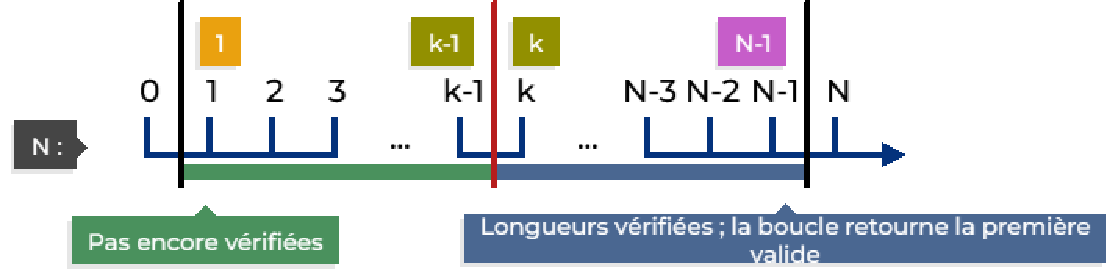
\includegraphics[width=1\textwidth]{invariant-1.pdf}
    \caption{Invariant graphique SP1}
\end{figure}

\subsection{SP2:}
\textbf{Invariant formel:} \\
    $ T = T_0 \land N = N_0 \land k = k_0$ \\
    $\land$ \\
    $0 \leq i < k$ \\
    $\land$ \\
    $T[i] = T[N - k + i]$ \\

\begin{figure}[h]
    \centering
    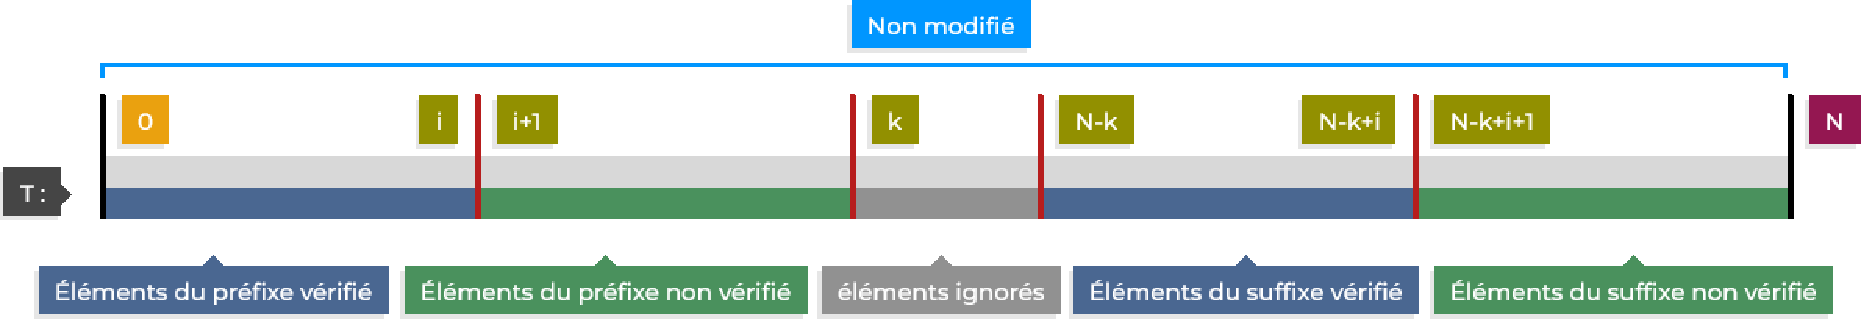
\includegraphics[width=1\textwidth]{invariant-2.pdf}
    \caption{Invariant graphique SP2}
\end{figure}



% !TEX root = ./main.tex
%%%%%%%%%%%%%%%%%%%%%%%%%%%%%%%%%%%%%%%%%%%%%%%%%%%%%%%%%%%%%%%%%%%%%%%%%%%%%%%%%%%%%%%%%%
% Justifiez, dans cette section, chacune de vos implémentations récursives à l'aide des  %
% 3 étapes vues au cours (cfr. Chap. 4)                                                  %
%%%%%%%%%%%%%%%%%%%%%%%%%%%%%%%%%%%%%%%%%%%%%%%%%%%%%%%%%%%%%%%%%%%%%%%%%%%%%%%%%%%%%%%%%%
\section{Implémentations Récursives}\label{recursivite}
%%%%%%%%%%%%%%%%%%%%%%%%%%%%%%%%%%%%%

Définition récursive:


course\_get\_escales\_count(course) = \\$
                \begin{cases}
                    return\ 0; & \text{if } course == NULL \\
                    return\ course\_get\_escales\_count(course->next) + 1; & \text{otherwise}
                \end{cases} $
\\

course\_get\_stages\_count(course) = \\$
                \begin{cases}
                    return\ 0; & \text{if } course == NULL \\
                    return\ 0; & \text{if } course->next == NULL \\
                    return\ course\_get\_stages\_count(course->next) + 1; & \text{otherwise}
                \end{cases} $
\\

course\_total\_time(course) = \\$
                \begin{cases}
                    return\ 0; & \text{if } course == NULL \\
                    return\ (\\
                    course\_total\_time(course->next) +\\
                    escale\_get\_best\_time(course->escale)\\
                    ); & \text{otherwise}
                \end{cases} $
\\

course\_best\_time\_at(course, index) = \\$
                \begin{cases}
                    return\ escale\_get\_best\_time(course->escale); & \text{if } index == 0 \\
                    return\ course\_best\_time\_at(course->next, index - 1); & \text{otherwise}
                \end{cases} $
\\

course\_append(course, escale) = \\$
                \begin{cases}
                    course = malloc(sizeof(Course)); \\
                    course->escale = escale; \\
                    course->next = NULL; \\
                    return\ course; & \text{if } course == NULL \\
                    \\
                    course->next = course\_append(course->next, escale);\\
                    return\ course; & \text{otherwise}
                \end{cases} $
\\

course\_pop(course) = \\$
                \begin{cases}
                    free(course->escale); \\
                    free(course); \\
                    return\ NULL; & \text{if } course->next == NULL \\
                    \\
                    course->next = course_pop(course->next);\\
                    return\ course; & \text{otherwise}
                \end{cases} $
\\

course\_free(course) = \\$
                \begin{cases}
                    return; & \text{if } course->next == NULL \\
                    \\
                    course\_free(course->next); \\
                    free(course->escale); \\
                    free(course); & \text{otherwise}
                \end{cases} $
\\

course\_last(course) = \\$
                \begin{cases}
                    return\ course; & \text{if } course->next == NULL \\
                    \\
                    return\ course\_last(course->next); & \text{otherwise}
                \end{cases} $


% !TEX root = ./main.tex
%%%%%%%%%%%%%%%%%%%%%%%%%%%%%%%%%%%%%%%%%%%%%%%%%%%%%%%%%%%%%%%%%%%%%%%%%%%%%%%%%%%%%%%%%%
% Dans cette section, vous devez étudier complètement la complexité de votre code.       %
% Soyez le plus formel (i.e., mathématique) possible.                                    %
%%%%%%%%%%%%%%%%%%%%%%%%%%%%%%%%%%%%%%%%%%%%%%%%%%%%%%%%%%%%%%%%%%%%%%%%%%%%%%%%%%%%%%%%%%
\section{Complexité}\label{complexite}
%%%%%%%%%%%%%%%%%%%%

\textbf{Complexité de \texttt{pref\_equal\_suff}}:
\begin{itemize}
    \item Complexité exacte:\\
        $ T_1(k) = 1 + (k+1) + k + k + 1 = 3k + 3$\\
    \item Asymptotique:\\
        $ T_1(k) \in \mathcal{O}(k) $
\end{itemize}

\textbf{Complexité de \texttt{prefixe\_suffixe}}:
\begin{itemize}
    \item Complexité exacte:\\
        \[
        T_2(N) = 1 + \sum_{k=N-1}^{1} [3 + T_1(k)] + 1
        = 2 + 3 \sum_{k=N-1}^{1} [3k + 6]
        = 2 + \frac{3(N-1)N}{2} + 6(N - 1)
        = \frac{3N^2 - 3N}{2} + 6N - 4
        \]
    \item Asymptotique:\\
        $ T_2(N) \in \mathcal{O}(N^2) $
\end{itemize}



% !TEX root = ./main.tex
%%%%%%%%%%%%%%%%%%%%%%%%%%%%%%%%%%%%%%%%%%%%%%%%%%%%%%%%%%%%%%%%%%%%%%%%%%%%%%%%%%%%%%%%%%
% Dans cette section, décrivez comment vous avez implémenté les différents tests         %
% unitaires                                                                              %
% Pensez à justifier vos choix.                                                          %
%%%%%%%%%%%%%%%%%%%%%%%%%%%%%%%%%%%%%%%%%%%%%%%%%%%%%%%%%%%%%%%%%%%%%%%%%%%%%%%%%%%%%%%%%%
\section{Tests Unitaires}\label{tests}
%%%%%%%%%%%%%%%%%%%%%%%%%

Les tests unitaires sont situés dans le dossier \texttt{test/} et utilisent le framework \texttt{seatest}.
Pour chaque implémentation (\texttt{course\_liste} et \texttt{course\_tableau}), deux fonctions principales sont testées :

\begin{itemize}
    \item \texttt{test\_course\_append} : vérifie que l'ajout d'escales modifie correctement le nombre d'escales dans la course.
    \item \texttt{test\_course\_total\_time} : vérifie que la somme des temps des escales est correcte après modification des temps et suppression d'éléments.
\end{itemize}

Les assertions utilisées sont \texttt{assert\_ulong\_equal} pour les entiers et \texttt{assert\_double\_equal} pour les valeurs réelles.

\textbf{Justification des choix :}
Les tests ciblent les opérations principales et les cas limites.


\textbf{Limite :}
Seules les fonctions d'ajout et de calcul du temps total sont testées.
Les autres fonctions publiques ne sont pas couvertes par les tests actuels.


% !TEX root = ./main.tex
%%%%%%%%%%%%%%%%%%%%%%%%%%%%%%%%%%%%%%%%%%%%%%%%%%%%%%%%%%%%%%%%%%%%%%%%%%%%%%%%%%%%%%%%%%
% Rédigez ici la conclusion de votre rapport.                                            %
%%%%%%%%%%%%%%%%%%%%%%%%%%%%%%%%%%%%%%%%%%%%%%%%%%%%%%%%%%%%%%%%%%%%%%%%%%%%%%%%%%%%%%%%%%
\section{Conclusion}\label{conclusion}
%%%%%%%%%%%%%%%%%%%%%

% C'est un cours difficile

Pour terminer ce rapport nous pouvons ajouter que nous avons réussi à créer un algorithme
en C cappable de trouver le plus long préfixe qui est aussi un suffixe d'une liste donnée.
Et tout cela en respectant les contraintes données tel que l'utilisation exclusives des
boucles while et l'abscence de l'utilisation de list intermédiaires.


%%%%%%%%%%%%%%%%%%%% FIN DE LA ZONE PROTÉGÉE %%%%%%%%%%%%%%%%%%%%

\end{document}
